\chapter{Moltiplicatori di Lagrange e principio di Hamilton}
\section{Massimi e minimi vincolati di una funzione a valori reali}
Sia \(f:\mathbb{R}^n \to \mathbb{R}\) abbastanza liscia \(\left(\text{almeno } C^2(\mathbb{R}^n)\right)\). Voglio trovare i punti ottimi della funzione ristretta a
\[
S=\left\{\underline{x}\in\mathbb{R}^n:g(\underline{x})=0\right\}.
\]
Chiamo
\[
\widetilde{f}=f\big|_S:S\to\mathbb{R}
\qquad
\underline{x}\mapsto f(\underline{x})
\]

In generale \(\widetilde{f}\) non ha gli stessi punti critici di \(f\).

Il problema quindi diventa trovare i punti critici di \(\widetilde{f}\). Ci sono 2 possibilità

\[
\text{i) il vincolo è esprimibile come}
\]
\[
x_1=\widetilde{g}(x_2,\ldots,x_n)
\]

In questo caso posso cercare in modo standard gli ottimi della funzione
\[
\widetilde{f}:\mathbb{R}^{n-1}\to\mathbb{R}
\qquad
(x_2,\ldots,x_n)\mapsto f(x_1(x_2,\ldots,x_n),x_2,\ldots,x_n)
\]

\[
\text{ii) in generale posso cercare i punti critici della funzione}
\]
\[
f_\lambda(x_1,\ldots,x_n,\lambda)
=
f(x_1,\ldots,x_n,\lambda)
-
\lambda g(x_1,\ldots,x_n)
\]

Dove \(\lambda\) è detto moltiplicatore di Lagrange. Dobbiamo quindi risolvere il sistema

\[
\nabla f_\lambda=0
\Longleftrightarrow
\begin{cases}
\dfrac{\partial f}{\partial x_i}
-
\lambda
\dfrac{\partial g}{\partial x_i}
=0
\qquad \forall i=1,\ldots,n
\\[1em]
g(x_1,\ldots,x_n)=0
\end{cases}
\]

\begin{example}{}
\[
f:\mathbb{R}^2\to\mathbb{R}
\qquad
f(x,y)=x^2+by^2
\]

\[
y=ax+c
\Rightarrow
g(x,y)=y-ax-c=0
\]

\[
\text{i) ricavo } y=ax-c \text{ e sostituisco}
\]

\[
\widetilde{f}:\mathbb{R}\to\mathbb{R}
\qquad
\widetilde{f}(x,y(x))=x^2+b(ax+c)^2
\]

\[
\frac{d\widetilde{f}}{dx}
=
2x+2b(ax+c)a
=
0
\Rightarrow
\widetilde{x}
=
-\frac{abc}{1+a^2b}
\Rightarrow
\widetilde{y}
=
a\widetilde{x}+c
=
-\frac{a^2bc}{1+a^2b}+c
\]

\[
\text{(ii) } f_\lambda:\mathbb{R}^3\to\mathbb{R}
\qquad
f_\lambda=x^2+by^2-\lambda(y-ax-c)
\]

\[
\nabla f_\lambda
=
(2x+\lambda a,\ 2by-\lambda,\ -y+ax+c)
\]

\[
\Rightarrow
\begin{cases}
2x+\lambda a=0
\Rightarrow
2x+2aby=0
\Rightarrow
2x+2ab(ax+c)=0
\Rightarrow
2x+2a^2bx+2abc=0
\\
2by-\lambda=0
\Rightarrow
\lambda=2by
\\
y-ax-c=0
\Rightarrow
y=ax+c
\end{cases}
\]

\[
\Rightarrow
x=
\frac{-2abc}{2(1+a^2b)}
=
-\frac{abc}{1+a^2b}
\]

\[
\Rightarrow
y=
-\frac{a^2bc}{1+a^2b}
+c
\]
\end{example}

\subsubsection{Interpretazione geometrica dei moltiplicatori di Lagrange}
\begin{center}
    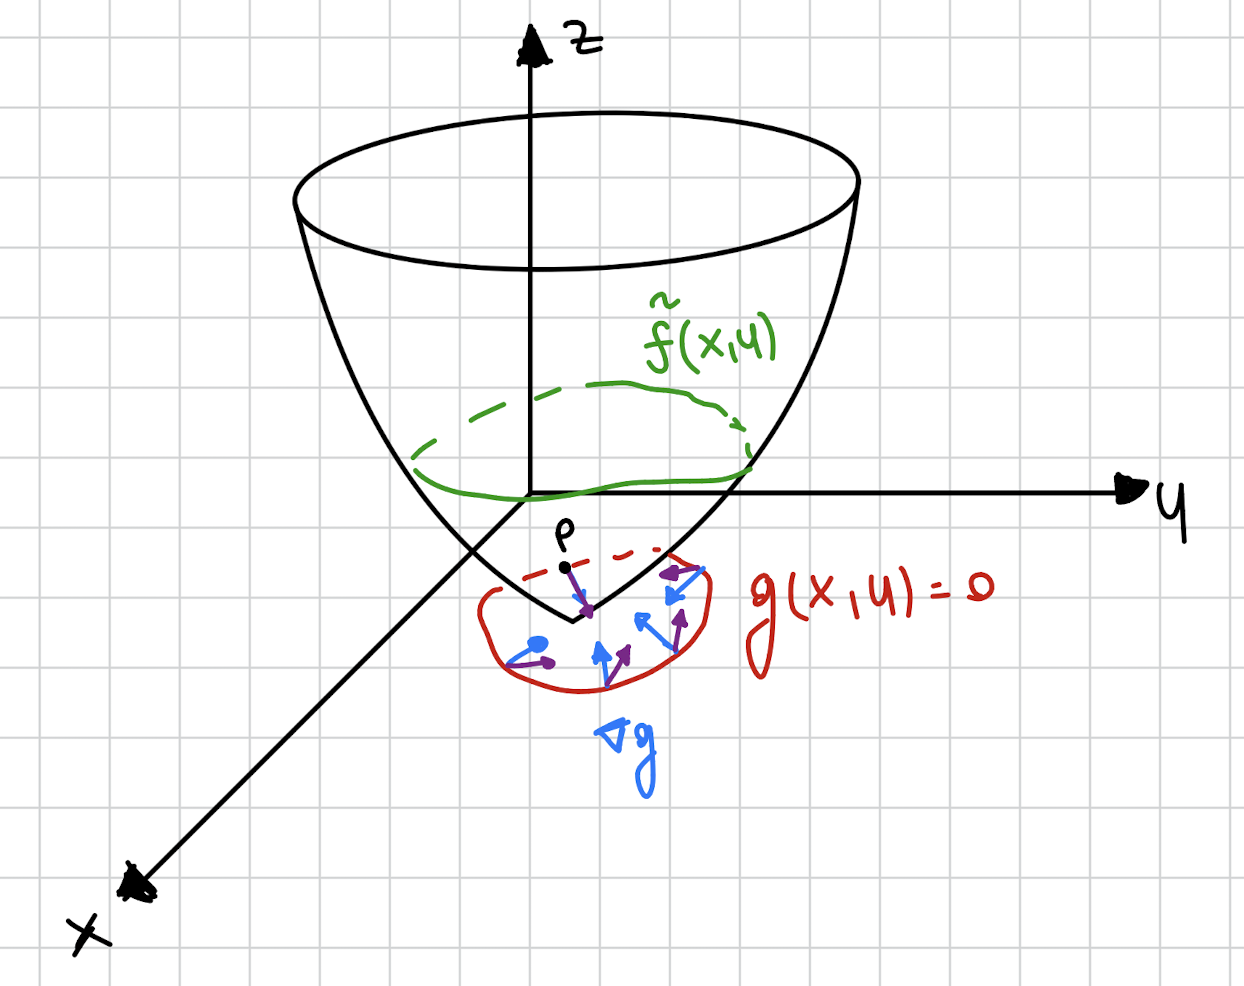
\includegraphics[scale=0.5]{immagini/molt-lagrange.png}
\end{center}

Sto chiedendo
\[
\nabla f_\lambda = \nabla f - \lambda \nabla g = 0
\Rightarrow
\nabla f = +\lambda \nabla g
\]
ovvero il minimo si ha nel punto in cui \(\nabla f\) e \(\nabla g\) sono paralleli. Infatti se così non fosse \(\nabla f\) avrebbe una componente parallela al vincolo e quindi seguendo quella direzione la funzione migliorerebbe. In figura il punto \(P\) è di ottimo.
\subsubsection{Significato fisico dei moltiplicatori di Lagrange}
Ci domandiamo che significato fisico abbia il moltiplicatore di Lagrange in un sistema meccanico.
\begin{example}{}
\[
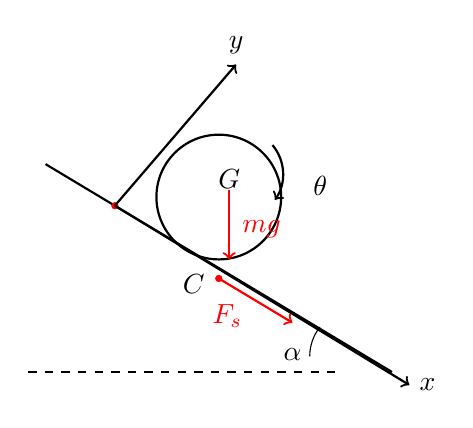
\begin{tikzpicture}[scale=1.1]
  % piano inclinato
  \draw[thick] (-2,1.2) -- (2,-1.2);
  \draw[dashed] (-2.2,-1.2) -- (1.4,-1.2);

  % assi
  \fill[red] (-1.2,0.72) circle (1.2pt);
  \draw[->,thick] (-1.2,0.72) -- (0.2,2.35) node[above] {$y$};
  \draw[->,thick] (-1.2,0.72) -- (2.2,-1.35) node[right] {$x$};

  % disco
  \draw[thick] (0,0.82) circle (0.72);
  \node at (0.12,1.03) {$G$};

  % centro e contatto
  \fill[red] (0,-0.12) circle (1.2pt);
  \node[left] at (-0.05,-0.18) {$C$};

  % mg
  \draw[->,red,thick] (0.12,0.9) -- (0.12,0.1);
  \node[red,right] at (0.16,0.45) {$mg$};

  % forza tangenziale
  \draw[->,red,thick] (0,-0.12) -- (0.85,-0.63);
  \node[red] at (0.1,-0.55) {$F_s$};

  % angolo alpha
  \draw (1.05,-1.02) arc[start angle=180,end angle=142,radius=0.55];
  \node at (0.85,-1.0) {$\alpha$};

  % freccia theta
  \draw[->,thick] (0.62,1.42) arc[start angle=40,end angle=-35,radius=0.52];
  \node[right] at (0.98,0.95) {$\theta$};
\end{tikzpicture}
\]

Il disco è soggetto ad un puro rotolamento

\[
x_G=R\theta
\qquad
\Rightarrow
\qquad
g(x_G,\theta)=x_G-R\theta
\qquad
\Rightarrow
\qquad
g(x_G,\theta)=0
\]

\[
T=\frac{m\dot{x}_G^2}{2}+\frac{mR^2}{2}\frac{\dot{\theta}^2}{2}
\qquad
V=mg\,x_G\sin\alpha
\qquad
\mathcal{L}=\frac{m\dot{x}_G^2}{2}+\frac{mR^2}{2}\frac{\dot{\theta}^2}{2}+mg\,x_G\sin\alpha
\]

\[
\mathcal{L}_\lambda=
\frac{m\dot{x}_G^2}{2}
+
\frac{mR^2}{2}\frac{\dot{\theta}^2}{2}
+
mg\,x_G\sin\alpha
-
\lambda(x_G-R\theta)
\]

\[
\begin{cases}
\dfrac{d}{dt}\dfrac{\partial\mathcal{L}}{\partial \dot{x}_G}-\dfrac{\partial\mathcal{L}}{\partial x_G}
=
-\lambda\dfrac{\partial g}{\partial x_G}
\\[1em]
\dfrac{d}{dt}\dfrac{\partial\mathcal{L}}{\partial \dot{\theta}}-\dfrac{\partial\mathcal{L}}{\partial \theta}
=
-\lambda\dfrac{\partial g}{\partial \theta}
\\[1em]
x_G=R\theta
\end{cases}
\qquad
\Rightarrow
\qquad
\begin{cases}
m\ddot{x}_G=mg\sin\alpha-\lambda
\\[0.6em]
\dfrac{mR^2}{2}\ddot{\theta}=\lambda R
\\[0.6em]
x_G=R\theta
\end{cases}
\]

\[
\Rightarrow
\begin{cases}
\lambda=\dfrac{mR\ddot{\theta}}{2}
\\[0.8em]
m\ddot{x}_G+\dfrac{mR}{2}\ddot{\theta}=mg\sin\alpha
\\[0.8em]
\dfrac{3}{2}mR\ddot{\theta}=mg\sin\alpha
\Rightarrow
\ddot{\theta}=\dfrac{2g\sin\alpha}{3R}
\end{cases}
\]

Assumo \(\dot{\theta}(0)=\theta(0)=0\). Allora

\[
\theta(t)=\frac{t^2}{3}\frac{\sin\alpha}{R}g
\]

Inoltre
\[
\lambda(t)=\frac{mR}{2}\cdot\frac{2}{3}\frac{\sin\alpha}{R}g
=
\frac{m\sin\alpha\, g}{3}
\]

Applichiamo la seconda cardinale con polo \(G\).

\[
\frac{d}{dt}\left(\frac{mR^2}{2}\dot{\theta}\,\hat{k}\right)
=
-R\hat{\jmath}\wedge F_s\hat{\imath}
=
+RF_s\hat{k}
\Rightarrow
\]

\[
\Rightarrow
RF_s=\frac{mR^2}{2}\ddot{\theta}
\Rightarrow
F_s=\frac{mR}{2}\ddot{\theta}
=
\lambda(t)
\]

\(\lambda\) è quindi la reazione vincolare tangente al vincolo descritto dalla coordinata libera.
\end{example}

\section{Derivate generalizzate (funzionali o variazionali)}
Consideriamo \((X,\|\cdot\|_X)\), \((Y,\|\cdot\|_Y)\) spazi vettoriali normati.
\begin{definition}{}


Sia \(r:X\to Y\). Diciamo che \(r\) è o-piccolo di \(x\in X\) e scriviamo
\[
r(x)=o(\|x\|_X)
\]
se
\[
\frac{\|r(x)\|_Y}{\|x\|_X}\longrightarrow 0
\]
per un determinato limite.
\end{definition}

\begin{definition}{}
Considero \(G:X\to Y\). Diciamo che \(G\) è differenziabile in \(x\in X\) se esiste un operatore lineare \(DG:X\to Y\) dipendente da \(x\) tale che
\[
G(x+\delta x)=G(x)+\left\langle DG\big|_x,\delta x\right\rangle+o(\|\delta x\|_X), \quad \forall \delta x \in X
\]
\end{definition}
La nozione di derivata appena definita generalizza quella classica di derivata o differenziale euclidei.
\begin{example}{}
\[
X=Y=\mathbb{R}
\qquad
\text{funzione}
\qquad
f=G:\mathbb{R}\to\mathbb{R}
\]

\[
f(x+\delta x)
=
f(x)+\langle f'(x),\delta x\rangle+o(\|\delta x\|)
=
f(x)+f'(x)\delta x+o(\|\delta x\|)
\]

\[
X=\mathbb{R}^n
\qquad
Y=\mathbb{R}
\qquad
f(\underline{x}+\delta\underline{x})
=
f(\underline{x})
+
\left\langle \nabla f\big|_{\underline{x}},\delta\underline{x}\right\rangle
+
o(\|\delta\underline{x}\|)
=
\]
\[
=
f(\underline{x})
+
\nabla f^T\cdot \delta\underline{x}
+
o(\|\delta\underline{x}\|)
\]

\[
X=Y=\mathbb{R}^{n,n}
\qquad
G:\mathbb{R}^{n,n}\to\mathbb{R}^{n,n}
\qquad
G(A)=A^2
\Rightarrow
DG\big|_A\cdot \delta A
=
A\delta A+\delta A\cdot A
\]

\[
G(A+\delta A)
=
G(A)
+
DG\big|_A\cdot \delta A
+
o(\|\delta A\|)
\]
\end{example}
\begin{example}{}
\[
X=\mathbb{R}^{3,3}
\qquad
Y=\mathbb{R}
\]

\[
G(A)=\det(A)
\Rightarrow
G(A+\delta A)
=
G(A)
+
DG\big|_A\,\delta A
+
o(\|A\|)
\]

Con un calcolo non banale si trova che
\[
DG\big|_A\cdot \delta A
=
\det A\cdot \operatorname{tr}\left(A^{-1}\delta A\right)
\]
\end{example}

\section{Principio di Hamilton}

Illustriamo un metodo alternativo per ottenere le equazioni di Lagrange.

Sia \(\mathcal{Y}\) lo spazio delle curve nello spazio delle configurazioni di estremi \(\underline{q}_1,\underline{q}_2\). Il seguente principio è equivalente al principio di Newton ed è detto principio di Hamilton.

Per andare da uno stato \(\underline{q}_1\) ad uno stato \(\underline{q}_2\) nello spazio delle fasi un sistema meccanico segue la traiettoria che rende stazionario il funzionale

\[
H(\underline{q},\dot{\underline{q}}):\mathcal{Y}\to\mathbb{R}
\qquad
H(\underline{q},\dot{\underline{q}})
=
\int_{t_1}^{t_2}\mathcal{L}(\underline{q},\dot{\underline{q}})\,dt
\]

\[
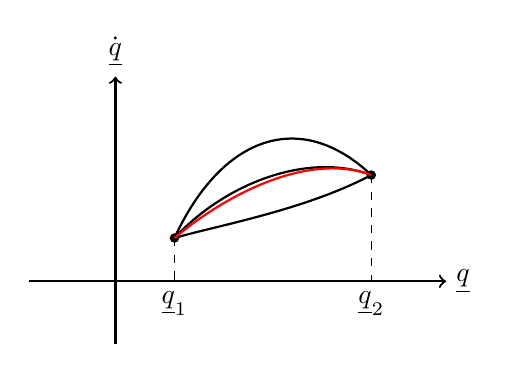
\begin{tikzpicture}[scale=1]
  \draw[->, thick] (-1.1,0) -- (4.2,0) node[right] {\(\underline{q}\)};
  \draw[->, thick] (0,-0.8) -- (0,2.6) node[above] {\(\dot{\underline{q}}\)};

  \coordinate (A) at (0.75,0.55);
  \coordinate (B) at (3.25,1.35);

  \filldraw[black] (A) circle (1.5pt);
  \filldraw[black] (B) circle (1.5pt);

  \draw[dashed] (A) -- (0.75,0);
  \draw[dashed] (B) -- (3.25,0);

  \node[below] at (0.75,0) {\(\underline{q}_1\)};
  \node[below] at (3.25,0) {\(\underline{q}_2\)};

  \draw[thick] (A) .. controls (1.35,1.85) and (2.35,2.20) .. (B);
  \draw[thick] (A) .. controls (1.40,1.25) and (2.45,1.65) .. (B);
  \draw[thick] (A) .. controls (1.25,0.70) and (2.40,0.90) .. (B);
  \draw[thick, red] (A) .. controls (1.40,1.10) and (2.45,1.65) .. (B);
\end{tikzpicture}
\]

La derivata generalizzata è

\[
\left\langle DH,(\delta\underline{q},\delta\dot{\underline{q}})\right\rangle
=
\delta \int_{t_1}^{t_2}\mathcal{L}(\underline{q},\dot{\underline{q}})\,dt
=
\int_{t_1}^{t_2}
\left(
\sum_i \frac{\partial \mathcal{L}}{\partial q_i}\delta q_i
+
\sum_i \frac{\partial \mathcal{L}}{\partial \dot{q}_i}\delta\dot{q}_i
\right)dt
\]

Stiamo trovando un punto di stazionarietà di \(H\) ovvero poniamo

\[
DH=0
\Longleftrightarrow
\left\langle DH,(\delta\underline{q},\delta\dot{\underline{q}})\right\rangle=0
\qquad
\forall(\delta\underline{q},\delta\dot{\underline{q}})
\]

Fissiamo \((\delta\underline{q},\delta\dot{\underline{q}})\) arbitrarie

\[
\int_{t_1}^{t_2}
\left(
\sum_i \frac{\partial \mathcal{L}}{\partial q_i}\delta q_i
+
\sum_i \frac{\partial \mathcal{L}}{\partial \dot{q}_i}\delta\dot{q}_i
\right)dt
=0
\]

Osserviamo
\[
\frac{d}{dt}\delta q_i=\delta\dot{q}_i
\]
allora

\[
\int_{t_1}^{t_2}
\left(
\sum_i \frac{\partial \mathcal{L}}{\partial q_i}\delta q_i
+
\sum_i \frac{\partial \mathcal{L}}{\partial \dot{q}_i}\frac{d}{dt}\delta q_i
\right)dt
=0
\]

Integriamo per parti l'ultimo termine

\[
\int_{t_1}^{t_2}
\left(
\sum_i \frac{\partial \mathcal{L}}{\partial q_i}\delta q_i
-
\sum_i \frac{d}{dt}\frac{\partial \mathcal{L}}{\partial \dot{q}_i}\delta q_i
\right)dt
+
\sum_i
\left[
\frac{\partial \mathcal{L}}{\partial \dot{q}_i}\delta q_i
\right]_{t_1}^{t_2}
=0
\]

Ora \(\delta\underline{q}(t_1)=\delta\underline{q}(t_2)=0\). Infatti consideriamo la curva

\[
(\underline{q}(t)+\delta\underline{q}(t),\dot{\underline{q}}(t)+\delta\dot{\underline{q}}(t)).
\]
Voglio che

\[
\underline{q}(t_i)+\delta\underline{q}(t_i)
=
\underline{q}_i
=
\underline{q}(t_i)
\Rightarrow
\delta\underline{q}(t_i)=0
\qquad
\forall i=1,2
\]

\[
\int_{t_1}^{t_2}
\sum_i
\left(
\frac{\partial \mathcal{L}}{\partial q_i}
-
\frac{d}{dt}\frac{\partial \mathcal{L}}{\partial \dot{q}_i}
\right)
\delta q_i\,dt
=0
\qquad
\forall \delta\underline{q}
\]

\[
\Rightarrow
\frac{d}{dt}\frac{\partial \mathcal{L}}{\partial \dot{q}_i}
=
\frac{\partial \mathcal{L}}{\partial q_i}
\qquad
\forall i
\]

per il lemma fondamentale del calcolo delle variazioni

Consideriamo un sistema meccanico con coordinate lagrangiane \([q_i]\) tra loro dipendenti e legate tra loro dal vincolo olonomo
\[
g(q_1,\ldots,q_n)=0
\]

Il moto è determinato dalla stazionarietà del funzionale

\[
H:\mathcal{Y}\to\mathbb{R}
\qquad
H(\underline{q},\dot{\underline{q}})
=
\int_{t_1}^{t_2}
\left(
\mathcal{L}(\underline{q},\dot{\underline{q}})
-
\lambda g(\underline{q})
\right)dt
\]

\[
\left\langle DH,(\delta\underline{q},\delta\dot{\underline{q}})\right\rangle
=
\delta H(\underline{q},\dot{\underline{q}})
=
\int_{t_1}^{t_2}
\left[
\sum_i \frac{\partial \mathcal{L}}{\partial q_i}\cdot \delta q_i
+
\sum_i \frac{\partial \mathcal{L}}{\partial \dot{q}_i}\cdot \delta\dot{q}_i
-
\lambda\sum_i \frac{\partial g}{\partial q_i}\cdot \delta q_i
\right]dt
\]

Trovo un punto di stazionarietà di \(H\)

\[
\int_{t_1}^{t_2}
\left[
\sum_i \frac{\partial \mathcal{L}}{\partial q_i}\cdot \delta q_i
+
\sum_i \frac{\partial \mathcal{L}}{\partial \dot{q}_i}\cdot \delta\dot{q}_i
-
\lambda\sum_i \frac{\partial g}{\partial q_i}\cdot \delta q_i
\right]dt
\]

\[
\Rightarrow
\int_{t_1}^{t_2}
\left[
\sum_i \frac{\partial \mathcal{L}}{\partial q_i}\cdot \delta q_i
+
\sum_i \frac{\partial \mathcal{L}}{\partial \dot{q}_i}\cdot \frac{d}{dt}\delta q_i
-
\lambda\sum_i \frac{\partial g}{\partial q_i}\cdot \delta q_i
\right]dt
=0
\]

\[
\delta\dot{q}_i=\frac{d}{dt}\delta q_i
\]

\[
\Rightarrow
\int_{t_1}^{t_2}
\left[
\sum_i \frac{\partial \mathcal{L}}{\partial q_i}\cdot \delta q_i
-
\lambda \frac{\partial g}{\partial q_i}\cdot \delta q_i
-
\frac{d}{dt}\frac{\partial \mathcal{L}}{\partial \dot{q}_i}\cdot \delta q_i
\right]dt
+
\sum_i
\frac{\partial \mathcal{L}}{\partial \dot{q}_i}\delta q_i
\Big|_{t_1}^{t_2}
=0
\]

\[
\Rightarrow
\int_{t_1}^{t_2}
\sum_i
\left(
\frac{\partial \mathcal{L}}{\partial q_i}
-
\lambda\frac{\partial g}{\partial q_i}
-
\frac{d}{dt}\frac{\partial \mathcal{L}}{\partial \dot{q}_i}
\right)\delta q_i
=0
\qquad
\forall \delta\underline{q}
\]

\[
\Rightarrow
\frac{d}{dt}\frac{\partial \mathcal{L}}{\partial \dot{q}_i}
+
\lambda\frac{\partial g}{\partial q_i}
=
\frac{\partial \mathcal{L}}{\partial q_i}
\qquad
\forall i
\]

Le equazioni di Lagrange che ne derivano sono quindi

\[
\begin{cases}
\dfrac{d}{dt}\dfrac{\partial \mathcal{L}}{\partial \dot{q}_i}
-
\dfrac{\partial \mathcal{L}}{\partial q_i}
+
\lambda\dfrac{\partial g}{\partial q_i}
=0
\qquad
\forall i
\\[1em]
g(q_1,\ldots,q_n)=0
\end{cases}
\]

\section{Vincoli anolonomi}
Un vincolo si dice anolonomo se dipende dalla velocità ma
non è integrabile, cioè non è riscrivibile come vincolo olonomo
mediante integrazione

Ci limitiamo a studiare vincoli anolonomi della forma

\[
\underline{a}(\underline{q}) \cdot \dot{\underline{q}} = 0
\qquad \text{dove} \qquad
\underline{q} = \{q_1(t), \ldots, q_n(t)\}
\]

Si può dimostrare che questo implica la condizione sugli
spostamenti virtuali
\[
\underline{a}(\underline{q}) \cdot \delta \underline{q} = 0
\qquad \forall \delta \underline{q} \text{ ammissibile}.
\]

Nel ricavare le equazioni di Lagrange poco prima dell'ultimo
passaggio avevamo scritto

\[
\sum_j
\left(
\frac{d}{dt}\frac{\partial \mathcal{L}}{\partial \dot{q}_j}
-
\frac{\partial \mathcal{L}}{\partial q_j}
\right)
\delta q_j = 0
\qquad \forall \delta q_j. \qquad \text{(forze conservative in } \mathcal{L}\text{)}
\]


oppure
\[
\sum_j
\left(
\frac{d}{dt}\frac{\partial T}{\partial \dot{q}_j}
-
\frac{\partial T}{\partial q_j}
\right)
\delta q_j
=
Q_j \delta q_j
\qquad \forall \delta q_j
\qquad \text{(caso generale)}
\]

Appendiamo il vincolo anolonomo alla lagrangiana ottenuta
dal principio dei lavori virtuali.

\[
\sum_j
\left(
\frac{d}{dt}\frac{\partial T}{\partial \dot{q}_j}
-
\frac{\partial T}{\partial q_j}
\right)
\delta q_j
=
\sum_j Q_j \delta q_j
+
\sum_j \lambda
\left(
a_j(q) \cdot \delta q_j
\right)
\qquad \forall \delta q_j.
\]

\[
\Rightarrow
\frac{d}{dt}\frac{\partial T}{\partial \dot{q}_j}
-
\frac{\partial T}{\partial q_j}
=
Q_j + \lambda a_j(q)
\]

\begin{example}{}
Consideriamo un disco nello spazio che rotola su un piano di massa \(m\) e raggio \(R\)
Il disco giace nel piano \(\xi z\). Il disco è sempre in piedi non si
inclina. Il centro di massa del disco ha coordinate \((x_G,y_G,R)\).
\begin{center}
  \begin{tikzpicture}[scale=1,>=Stealth,line cap=round,line join=round]

% coordinate principali
\coordinate (O)  at (0,0);
\coordinate (Z)  at (0,5.2);
\coordinate (Y)  at (7.2,0);
\coordinate (X)  at (-3.4,-4.5);

\coordinate (C)  at (1.73,-1.55);
\coordinate (Xi) at ($(O)!3.0!(C)$);

\coordinate (G)  at (2.15,-0.55);

% assi neri
\draw[->, very thick] (O) -- (Z);
\draw[->, very thick] (O) -- (Y);
\draw[->, very thick] (O) -- (X);
\draw[->, very thick] (O) -- (Xi);

% etichette assi
\node[above right] at (Z) {$z$};
\node[right]       at (Y) {$y$};
\node[below left]  at (X) {$x$};
\node[below right] at (Xi) {$\xi$};

% segmento interno
\draw[very thick] (O) -- (C);

% disco / ellisse (non ruotata)
\draw[very thick] (G) ellipse [x radius=0.72, y radius=1.20];

% punti
\fill (C) circle (2.3pt);
\node[below] at (C) {$C$};

\fill (G) circle (2pt);
\node[left] at (G) {$G$};

% vettore k-hat dal polo
\draw[->, very thick, green!55!black] (O) -- ++(0,1.55);
\node[left, green!55!black] at (-0.75,0.95) {$\hat{k}$};

% vettori verdi applicati in G
\draw[->, very thick, green!55!black] (G) -- ++(0,2.60);
\draw[->, very thick, green!55!black] (G) -- ++(2.15,1.80);
\draw[->, very thick, green!55!black] (G) -- ++(2.10,-1.75);

\node[right, green!55!black] at (4.20,1.55) {$\hat{n}$};
\node[right] at (3.95,-1.05) {$\dot{x}_G$};

% arco nero per phi all'origine
\draw[very thick,->] (-0.55,-0.85) arc[start angle=-123,end angle=-40,radius=1.00];
\node at (-0.38,-1.55) {$\varphi$};

% freccia rossa in alto: rotazione antioraria attorno all'asse \varphi
\draw[->, very thick, red!80!black]
  ($(G)+(-0.28,2.11)$) arc[start angle=210,end angle=450,x radius=0.38,y radius=0.28];
\node[red!80!black] at ($(G)+(0.55,2.55)$) {$\varphi$};

% freccia rossa per theta
\draw[->, very thick, red!80!black]
  (3.10,0.95) arc[start angle=125,end angle=10,radius=0.82];
\node[red!80!black] at (4.08,0.42) {$\theta$};

\end{tikzpicture}
\end{center}


Uso la formula fondamentale del moto dei corpi rigidi, imponendo \(v_C=0\),
ovvero imponendo il puro rotolamento. Chiamo \(\hat{k}\) il versore
dell'asse \(z\) e \(\hat{n}\) il versore dell'asse di rotazione
\(\dot{\theta}\). Allora
\[
\omega=\dot{\varphi}\hat{k}+\dot{\theta}\hat{n}.
\]

\[
\dot{\underline{x}}_G
=
\omega \wedge (\underline{x}_G-\underline{x}_C)
=
(\dot{\varphi}\hat{k}+\dot{\theta}\hat{n})\wedge R\hat{k}
=
\dot{\theta}R\hat{n}\wedge\hat{k}
\]

Ora notiamo che
\[
\hat{n}=-\sin\varphi\,\hat{i}+\cos\varphi\,\hat{j},
\]
allora
\[
\dot{\underline{x}}_G
=
\dot{\theta}R
\left(
-\sin\varphi\,\hat{i}\wedge\hat{k}
+
\cos\varphi\,\hat{j}\wedge\hat{k}
\right)
=
+\dot{\theta}R\sin\varphi\,\hat{j}
+
\dot{\theta}R\cos\varphi\,\hat{i}
\]

ovvero
\[
\begin{cases}
\dot{x}_G=\dot{\theta}R\cos\varphi\\
\dot{y}_G=\dot{\theta}R\sin\varphi
\end{cases}
\]

Questa relazione non è integrabile ovvero il vincolo è anolonomo.

Possiamo riscrivere il vincolo come
\[
\begin{cases}
1\cdot \dot{x}_G-(R\cos\varphi)\dot{\theta}=0\\
1\cdot \dot{y}_G-(R\sin\varphi)\dot{\theta}=0
\end{cases}
\]

Studiamo il moto per inerzia del disco nel piano
\[
\underline{q}=\{x_G,y_G,\theta,\varphi\}
\]

Le 4 coordinate libere sono legate tra loro dai 2 vincoli anolonomi.

Il primo vincolo si può scrivere come
\[
\begin{pmatrix}
1\\
0\\
-R\cos\varphi\\
0
\end{pmatrix}
\cdot
\begin{pmatrix}
\dot{x}_G\\
\dot{y}_G\\
\dot{\theta}\\
\dot{\varphi}
\end{pmatrix}
=0
\]

Il secondo come
\[
\begin{pmatrix}
0\\
1\\
-R\sin\varphi\\
0
\end{pmatrix}
\cdot
\begin{pmatrix}
\dot{x}_G\\
\dot{y}_G\\
\dot{\theta}\\
\dot{\varphi}
\end{pmatrix}
=0
\]

\[
\Rightarrow
\quad
\underline{a}_1=(1,0,-R\cos\varphi,0)^T
\qquad
\underline{a}_2=(0,1,-R\sin\varphi,0)^T
\]

\[
T=
\frac{m}{2}\left(\dot{x}_G^2+\dot{y}_G^2\right)
+
\frac{I_\varphi \dot{\varphi}^2}{2}
+
I_\theta\frac{\dot{\theta}^2}{2}
=
\mathcal{L}
\]

Scrivo le equazioni di Lagrange con i vincoli
\[
\begin{cases}
m\ddot{x}_G=\lambda_1\cdot 1+\lambda_2\cdot 0=\lambda_1\\
m\ddot{y}_G=\lambda_1\cdot 0+\lambda_2\cdot 1=\lambda_2\\
I_\theta\ddot{\theta}
=
\lambda_1\cdot(-R\cos\varphi)+\lambda_2(-R\sin\varphi)
=
-\lambda_1R\cos\varphi-\lambda_2R\sin\varphi\\
I_\varphi\ddot{\varphi}=\lambda_1\cdot 0+\lambda_2\cdot 0=0
\end{cases}
\]

Le incognite sono \(x_G,y_G,\theta,\varphi,\lambda_1,\lambda_2\).
Ho quindi un sistema sottodeterminato. Aggiungo le equazioni dei vincoli.
\[
\begin{cases}
m\ddot{x}_G=\lambda_1\\
m\ddot{y}_G=\lambda_2\\
I_\theta\ddot{\theta}
=
-\lambda_1R\cos\varphi-\lambda_2R\sin\varphi\\
I_\varphi\ddot{\varphi}=0\\
\dot{x}_G=R\dot{\theta}\cos\varphi\\
\dot{y}_G=R\dot{\theta}\sin\varphi
\end{cases}
\]

Partiamo da \(I_\varphi\ddot{\varphi}=0\) con
\(\varphi(0)=0\), \(\dot{\varphi}(0)=\omega_\varphi\)
\[
\Rightarrow
\varphi(t)=\omega_\varphi t
\]

\[
\begin{cases}
m\ddot{x}_G=\lambda_1\\
m\ddot{y}_G=\lambda_2\\
I_\theta\ddot{\theta}
=
-\lambda_1R\cos(\omega_\varphi t)
-\lambda_2R\sin(\omega_\varphi t)\\
\dot{x}_G=R\dot{\theta}\cos(\omega_\varphi t)\\
\dot{y}_G=R\dot{\theta}\sin(\omega_\varphi t)
\end{cases}
\]

Derivo nel tempo la (5) e la (6)
\[
\ddot{x}_G
=
R\ddot{\theta}\cos(\omega_\varphi t)
-
R\dot{\theta}\omega_\varphi\sin(\omega_\varphi t)
\]
\[
\ddot{y}_G
=
R\ddot{\theta}\sin(\omega_\varphi t)
+
R\dot{\theta}\omega_\varphi\cos(\omega_\varphi t)
\]

Sostituisco in (1) e (2)
\[
\begin{cases}
mR\ddot{\theta}\cos(\omega_\varphi t)
-
mR\dot{\theta}\omega_\varphi\sin(\omega_\varphi t)
=
\lambda_1\\
mR\ddot{\theta}\sin(\omega_\varphi t)
+
mR\dot{\theta}\omega_\varphi\cos(\omega_\varphi t)
=
\lambda_2\\
I_\theta\ddot{\theta}
=
-\lambda_1R\cos(\omega_\varphi t)
-
\lambda_2R\sin(\omega_\varphi t)
\end{cases}
\]

Sostituisco \(\lambda_1,\lambda_2\) in (3)
\[
I_\theta\ddot{\theta}
=
-
\left(
mR\ddot{\theta}\cos(\omega_\varphi t)
-
mR\dot{\theta}\omega_\varphi\sin(\omega_\varphi t)
\right)
R\cos(\omega_\varphi t)
-
\left(
mR\ddot{\theta}\sin(\omega_\varphi t)
+
m\omega_\varphi R\dot{\theta}\cos(\omega_\varphi t)
\right)
R\sin(\omega_\varphi t)
\]

\[
\Rightarrow
\quad
I_\theta\ddot{\theta}=-mR^2\ddot{\theta}
\quad
\Rightarrow
\quad
\ddot{\theta}=0
\]

Imponendo \(\theta(0)=0\), \(\dot{\theta}(0)=\omega_\theta\) otteniamo
\[
\theta(t)=\omega_\theta t
\]

Possiamo quindi trovare \(\underline{x}_G\).

\[
\begin{cases}
\dot{x}_G=R\omega_\theta\cos(\omega_\varphi t)\\
\dot{y}_G=R\omega_\theta\sin(\omega_\varphi t)
\end{cases}
\Rightarrow
\begin{cases}
x_G
=
R\frac{\omega_\theta}{\omega_\varphi}\sin(\omega_\varphi t)+C_1\\
y_G
=
-R\frac{\omega_\theta}{\omega_\varphi}\cos(\omega_\varphi t)+C_2
\end{cases}
\]

Imponendo \(x_G(0)=0\), \(y_G(0)=0\)
\[
x_G
=
R\frac{\omega_\theta}{\omega_\varphi}\sin(\omega_\varphi t)
\]
\[
y_G
=
-R\frac{\omega_\theta}{\omega_\varphi}\cos(\omega_\varphi t)
+
R\frac{\omega_\theta}{\omega_\varphi}
\]
Il disco percorre quindi una circonferenza nel piano $xy$ di raggio $R\omega_{\theta}/\omega_{\varphi}$.
\end{example}


\begin{example}{}
  Studiamo il moto di un pattino su un piano inclinato.
  \begin{center}
    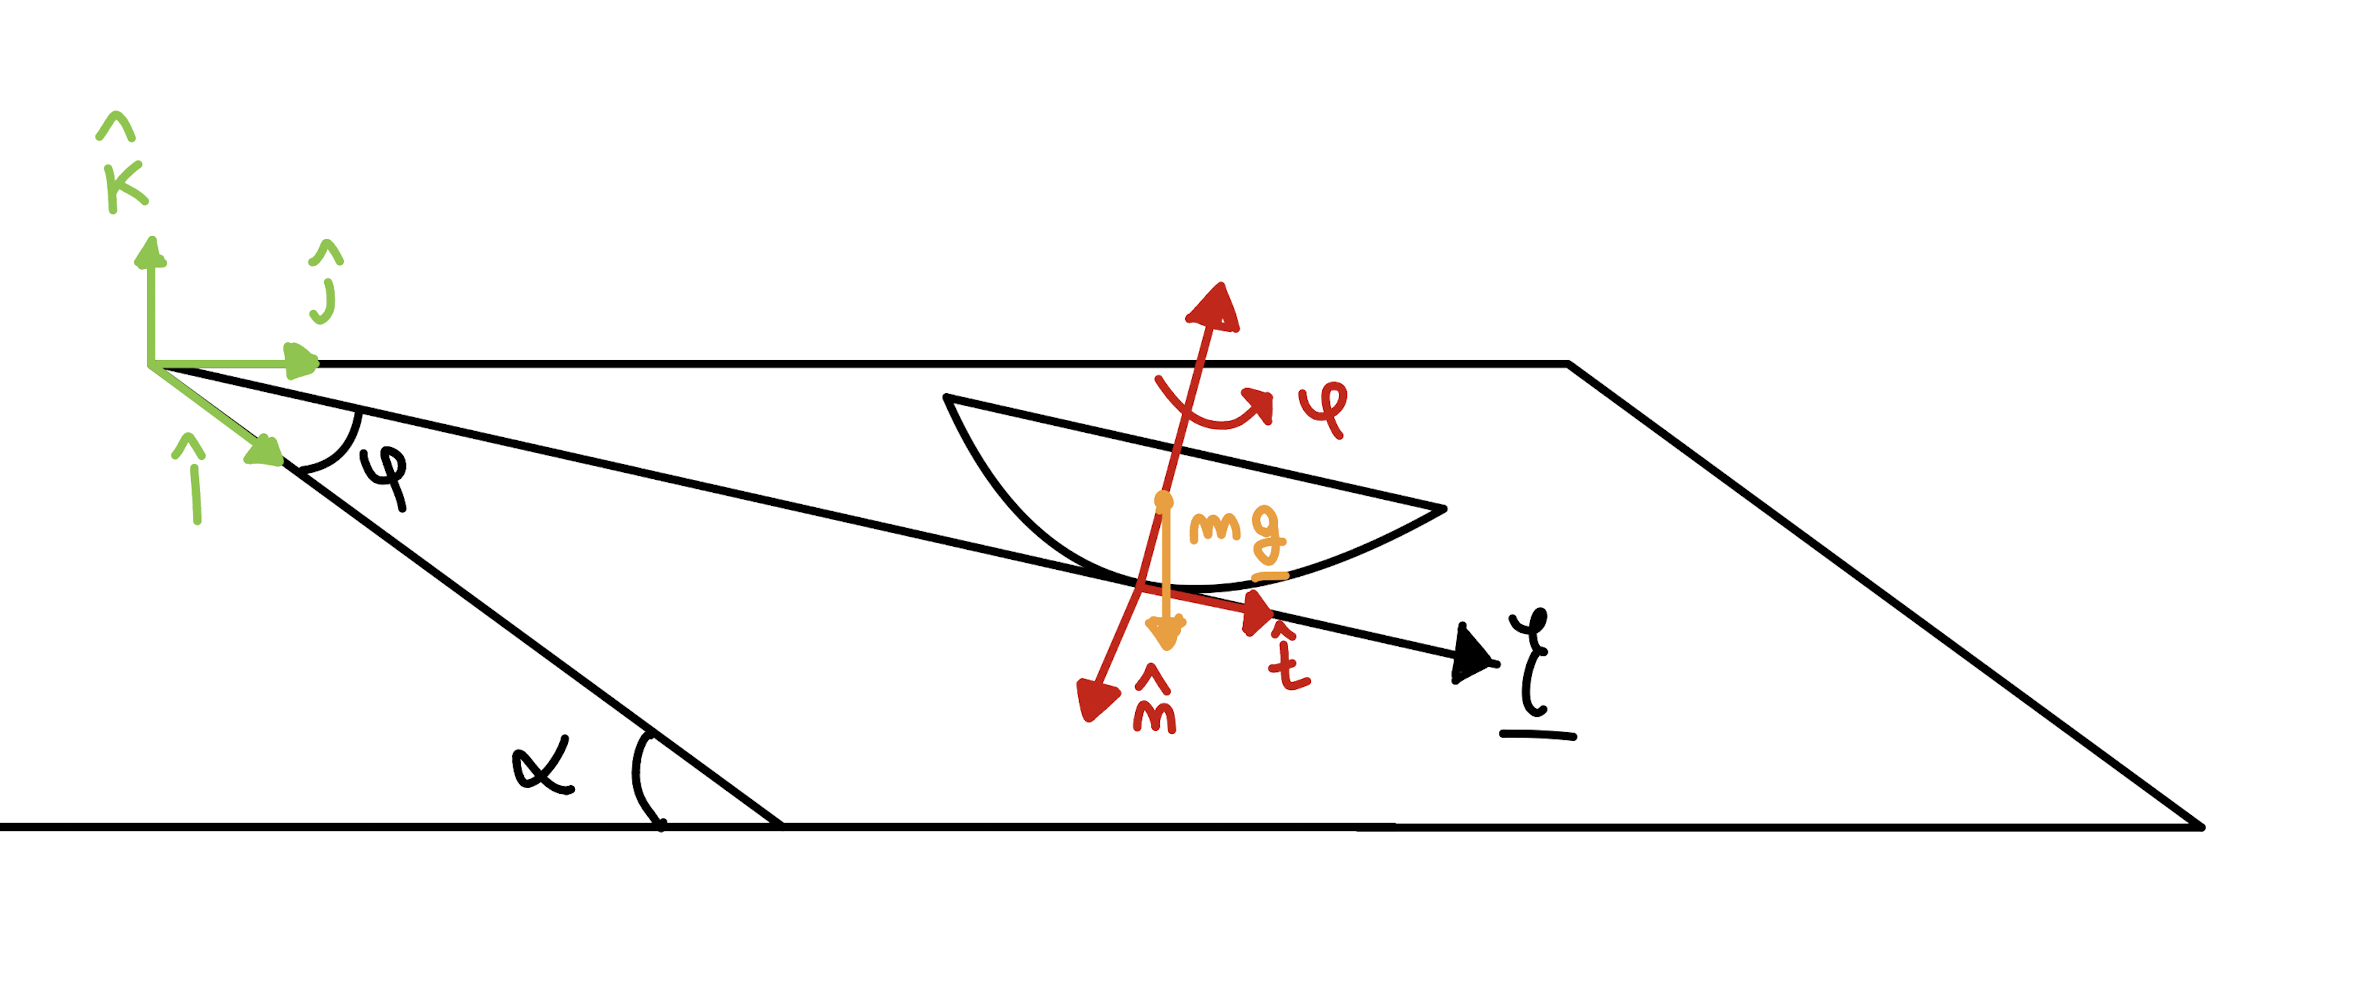
\includegraphics[scale=0.3]{immagini/pattino.png}
  \end{center}
Il pattino può solo avere componente della velocità lungo la propria direzione
(non può derapare). Il pattino sta nel piano verticale \((\hat{\xi},\hat{k})\)

\[
\hat{t}=
\begin{pmatrix}
\cos\varphi\\
\sin\varphi
\end{pmatrix}
\qquad
\hat{n}=
\begin{pmatrix}
+\sin\varphi\\
-\cos\varphi
\end{pmatrix}
\]

Posso scrivere il vincolo
\[
\dot{\underline{x}}_G\cdot \hat{n}=0
\Longleftrightarrow
\dot{x}_G\sin\varphi-\dot{y}_G\cos\varphi=0
\]

Il vincolo è anolonomo. Uso le coordinate libere
\((x_G,y_G,\varphi)\) dipendenti.

\[
T=
\frac{m\dot{x}_G^2}{2}
+
\frac{m\dot{y}_G^2}{2}
+
I\frac{\dot{\varphi}^2}{2}
\qquad
V=-mg\sin\alpha\, x_G
\]

\[
\mathcal{L}=T-V=
\frac{m\dot{x}_G^2}{2}
+
\frac{m\dot{y}_G^2}{2}
+
I\frac{\dot{\varphi}^2}{2}
+
mg\sin\alpha\, x_G
\]

Il vincolo può essere scritto nella forma

\[
\underbrace{
\begin{pmatrix}
-\sin\varphi\\
\cos\varphi\\
0
\end{pmatrix}
}_{\underline{a}}
\cdot
\begin{pmatrix}
\dot{x}_G\\
\dot{y}_G\\
\dot{\varphi}
\end{pmatrix}
=0
\]

Scrivo

\[
\frac{d}{dt}
\left(
\frac{\partial \mathcal{L}}{\partial \dot{q}_j}
\right)
-
\frac{\partial \mathcal{L}}{\partial q_j}
=
a_j\lambda
\qquad
\forall j
\]

ovvero

\[
\begin{cases}
m\ddot{x}_G-mg\sin\alpha=-\lambda\sin\varphi\\
m\ddot{y}_G=\lambda\cos\varphi\\
I\ddot{\varphi}=0\\
-\dot{x}_G\sin\varphi+\dot{y}_G\cos\varphi=0
\end{cases}
\]

Suppongo
\[
\varphi(0)=0
\qquad
\dot{\varphi}(0)=\omega
\Rightarrow
\varphi(t)=\omega t
\]

Utilizziamo l'integrale primo dell'energia dove
\[
x_G(0)=y_G(0)=0
\]
\[
\dot{x}_G(0)=\dot{y}_G(0)=0
\]

\[
\frac{m\dot{x}_G^2}{2}
+
\frac{m\dot{y}_G^2}{2}
+
I\frac{\omega^2}{2}
-
mgx_G\sin\alpha
=
I\frac{\omega^2}{2}
\]

\[
\begin{cases}
\frac{m}{2}\dot{x}_G^2
+
\frac{m}{2}\dot{y}_G^2
-
mg\sin\alpha\,x_G=0\\
\dot{x}_G\sin\varphi-\dot{y}_G\cos\varphi=0
\end{cases}
\Rightarrow
\begin{cases}
\frac{m}{2}\dot{x}_G^2
+
\frac{m}{2}\dot{x}_G^2\tg^2\varphi
-
mg\sin\alpha\,x_G=0\\
\dot{y}_G=\dot{x}_G\tg\varphi
\end{cases}
\]

\[
\frac{m}{2}\dot{x}_G^2
\left(
1+\tg^2\varphi
\right)
=
mg\sin\alpha\,x_G
\Rightarrow
\dot{x}_G^2
=
2g\sin\alpha\,x_G\cdot \cos^2\varphi
\]

\[
\Rightarrow
\dot{x}_G
=
\sqrt{2g\sin\alpha}\cos\varphi\sqrt{x_G}
\]

\[
\Rightarrow
\frac{\dot{x}_G}{\sqrt{x_G}}
=
\sqrt{2g\sin\alpha}\cos(\omega t)
\Rightarrow
\int
\frac{1}{\sqrt{x_G}}\,dx_G
=
\int
\sqrt{2g\sin\alpha}\cos(\omega t)\,dt
\]

\[
\Rightarrow
2\sqrt{x_G}
=
\sqrt{2g\sin\alpha}\frac{\sin(\omega t)}{\omega}
+
C
\]

Impongo
\[
x_G(0)=0
\]

\[
\Rightarrow
\sqrt{x_G}
=
\sqrt{\frac{g\sin\alpha}{2}}
\cdot
\frac{\sin(\omega t)}{\omega}
\Rightarrow
x_G
=
\frac{g\sin\alpha}{2}
\frac{\sin^2(\omega t)}{\omega^2}
\]

\[
\Rightarrow
\dot{x}_G
=
g\sin\alpha
\frac{\sin(\omega t)\cos(\omega t)}{\omega}
=
g\sin\alpha
\frac{\sin(2\omega t)}{2\omega}
\]

\[
\dot{y}_G
=
\tg\varphi\,\dot{x}_G
=
g\sin\alpha
\frac{\sin(2\omega t)}{2\omega}
\cdot
\tg(\omega t)
=
g\sin\alpha
\frac{\sin^2(\omega t)}{\omega}
=
\frac{g\sin\alpha}{\omega}
\cdot
\frac{1-\cos(2\omega t)}{2}
\]

Integrando \(y_G\) si ottiene

\[
\begin{cases}
x_G(t)
=
\frac{g\sin\alpha}{2\omega^2}
\frac{1-\cos(2\omega t)}{2}\\
y_G(t)
=
\frac{g\sin\alpha}{2\omega}
\left(
t-\frac{\sin(2\omega t)}{2\omega}
\right)
\end{cases}
\]
\begin{center}
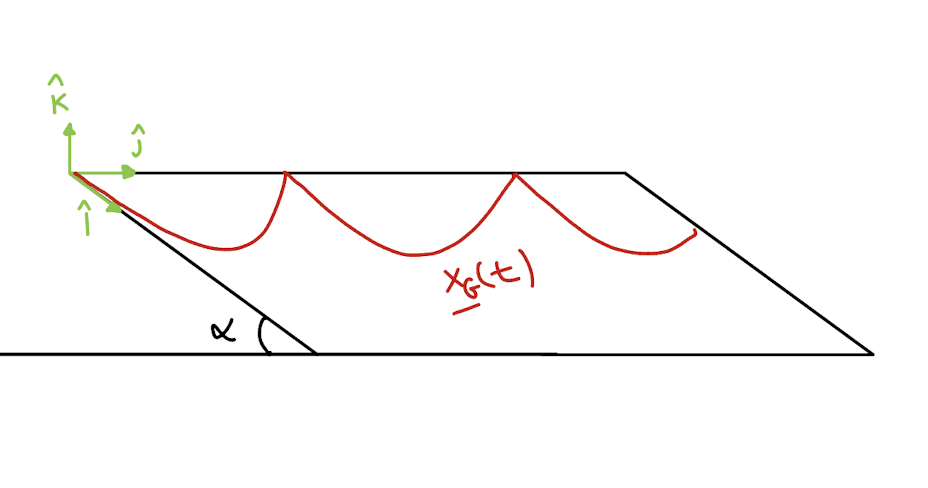
\includegraphics[scale=0.6]{immagini/pattino_1.png}
\end{center}

\end{example}
